% Auto-generated by the analysis pipeline — do not edit
% y > 0: Overreacts  |  y < 0: Underreacts
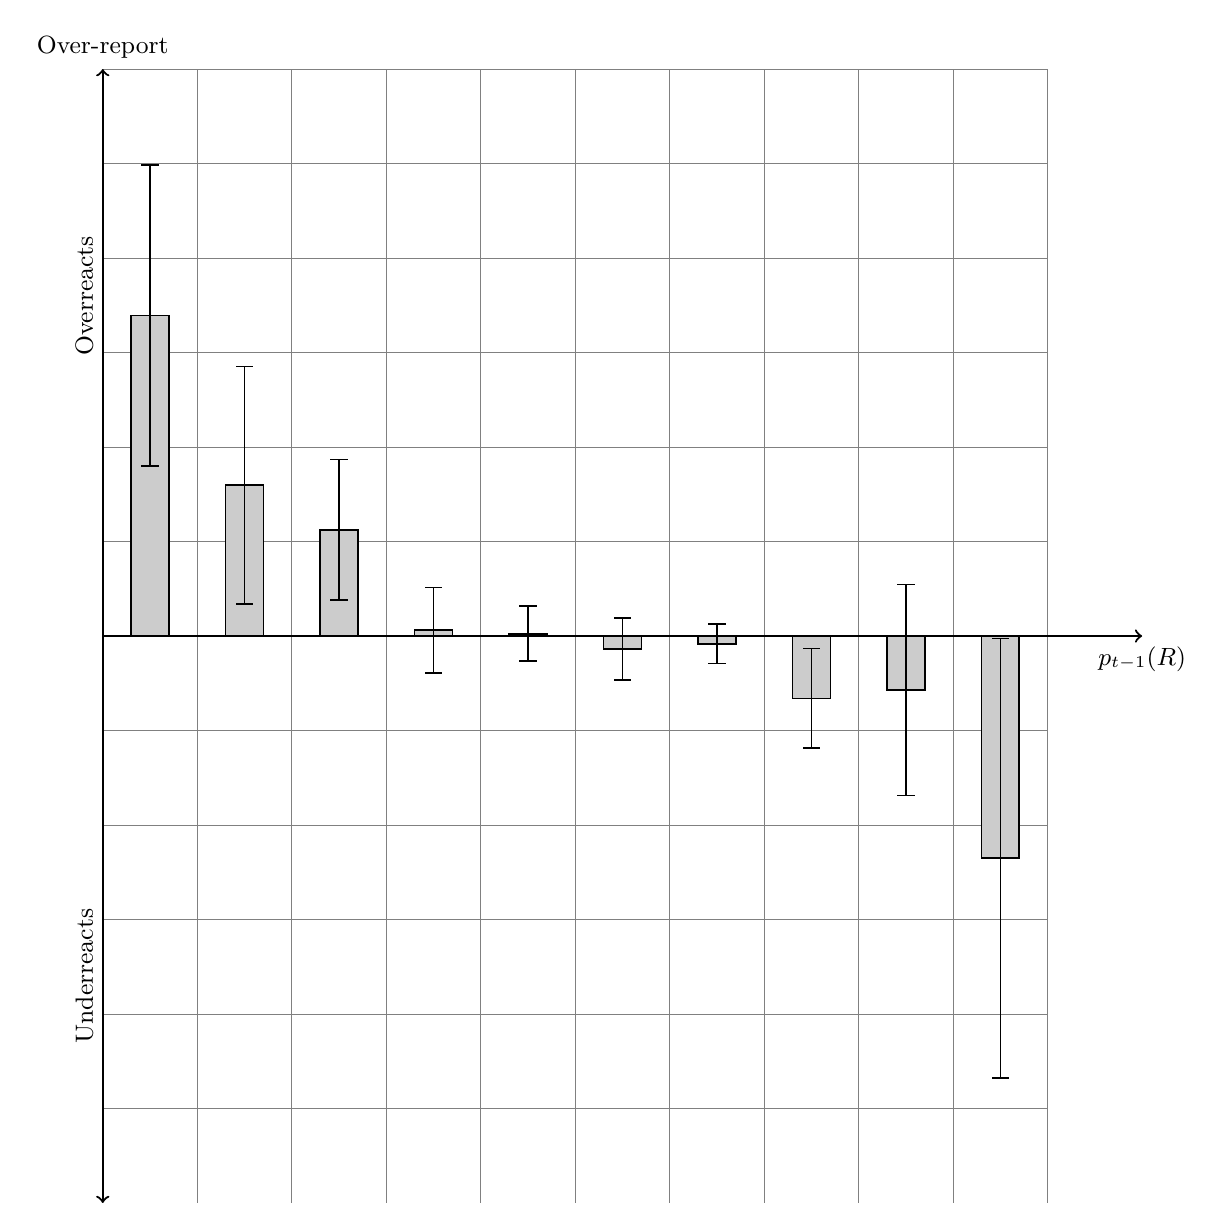
\begin{tikzpicture}[scale=12]
\draw[help lines,step=0.1] (0,-0.6) grid (1,0.6);
\filldraw[opaque,white!80!black] (0.03,0) rectangle (0.07,0.3392);
\draw[line width=0.6] (0.03,0) rectangle (0.07,0.3392);
\draw[line width=0.6,|-|] (0.05,0.1790) -- (0.05,0.4995);
\filldraw[opaque,white!80!black] (0.13,0) rectangle (0.17,0.1596);
\draw[line width=0.6] (0.13,0) rectangle (0.17,0.1596);
\draw[line width=0.6,|-|] (0.15,0.0328) -- (0.15,0.2863);
\filldraw[opaque,white!80!black] (0.23,0) rectangle (0.27,0.1123);
\draw[line width=0.6] (0.23,0) rectangle (0.27,0.1123);
\draw[line width=0.6,|-|] (0.25,0.0370) -- (0.25,0.1876);
\filldraw[opaque,white!80!black] (0.33,0) rectangle (0.37,0.0062);
\draw[line width=0.6] (0.33,0) rectangle (0.37,0.0062);
\draw[line width=0.6,|-|] (0.35,-0.0401) -- (0.35,0.0524);
\filldraw[opaque,white!80!black] (0.43,0) rectangle (0.47,0.0024);
\draw[line width=0.6] (0.43,0) rectangle (0.47,0.0024);
\draw[line width=0.6,|-|] (0.45,-0.0276) -- (0.45,0.0325);
\filldraw[opaque,white!80!black] (0.53,0) rectangle (0.57,-0.0136);
\draw[line width=0.6] (0.53,0) rectangle (0.57,-0.0136);
\draw[line width=0.6,|-|] (0.55,-0.0476) -- (0.55,0.0203);
\filldraw[opaque,white!80!black] (0.63,0) rectangle (0.67,-0.0084);
\draw[line width=0.6] (0.63,0) rectangle (0.67,-0.0084);
\draw[line width=0.6,|-|] (0.65,-0.0301) -- (0.65,0.0134);
\filldraw[opaque,white!80!black] (0.73,0) rectangle (0.77,-0.0660);
\draw[line width=0.6] (0.73,0) rectangle (0.77,-0.0660);
\draw[line width=0.6,|-|] (0.75,-0.1195) -- (0.75,-0.0125);
\filldraw[opaque,white!80!black] (0.83,0) rectangle (0.87,-0.0571);
\draw[line width=0.6] (0.83,0) rectangle (0.87,-0.0571);
\draw[line width=0.6,|-|] (0.85,-0.1696) -- (0.85,0.0554);
\filldraw[opaque,white!80!black] (0.93,0) rectangle (0.97,-0.2351);
\draw[line width=0.6] (0.93,0) rectangle (0.97,-0.2351);
\draw[line width=0.6,|-|] (0.95,-0.4683) -- (0.95,-0.0019);
\draw[line width=0.8,->]  (0,0) -- (1.1,0) node[below] {\small{$p_{t-1}(R)$}};
\draw[line width=0.8,<->] (0,-0.6) -- (0,0.6) node[above] {\small{Over-report}};
\draw (0,0.36) node[above,rotate=90] {\small{Overreacts}};
\draw (0,-0.36) node[above,rotate=90] {\small{Underreacts}};
% ADD THEORY CURVE BELOW
\end{tikzpicture}
